\hypertarget{residual-sac-ux4e0e-safe-residual-sac}{%
\section{Residual SAC 与 Safe Residual SAC}\label{residual-sac-ux4e0e-safe-residual-sac}}

V2--V5 不是四项并列贡献，而是一条逐步缩小假设空间的证据链。Direct PPO 先说明全量 actor 更新太容易漂移；Residual SAC 把改动限制在 Frozen AWAC 周围，却暴露 Q 排序和动作饱和问题；Safe Residual 修复了动作参数化之后仍然退化，排除了``只要 residual 足够小就安全''；反事实 branch 和 candidate ranker 改用真实仿真 outcome，最终又说明从局部视觉历史预测长时 gain/harm 本身就很难。

\begin{figure}
\centering
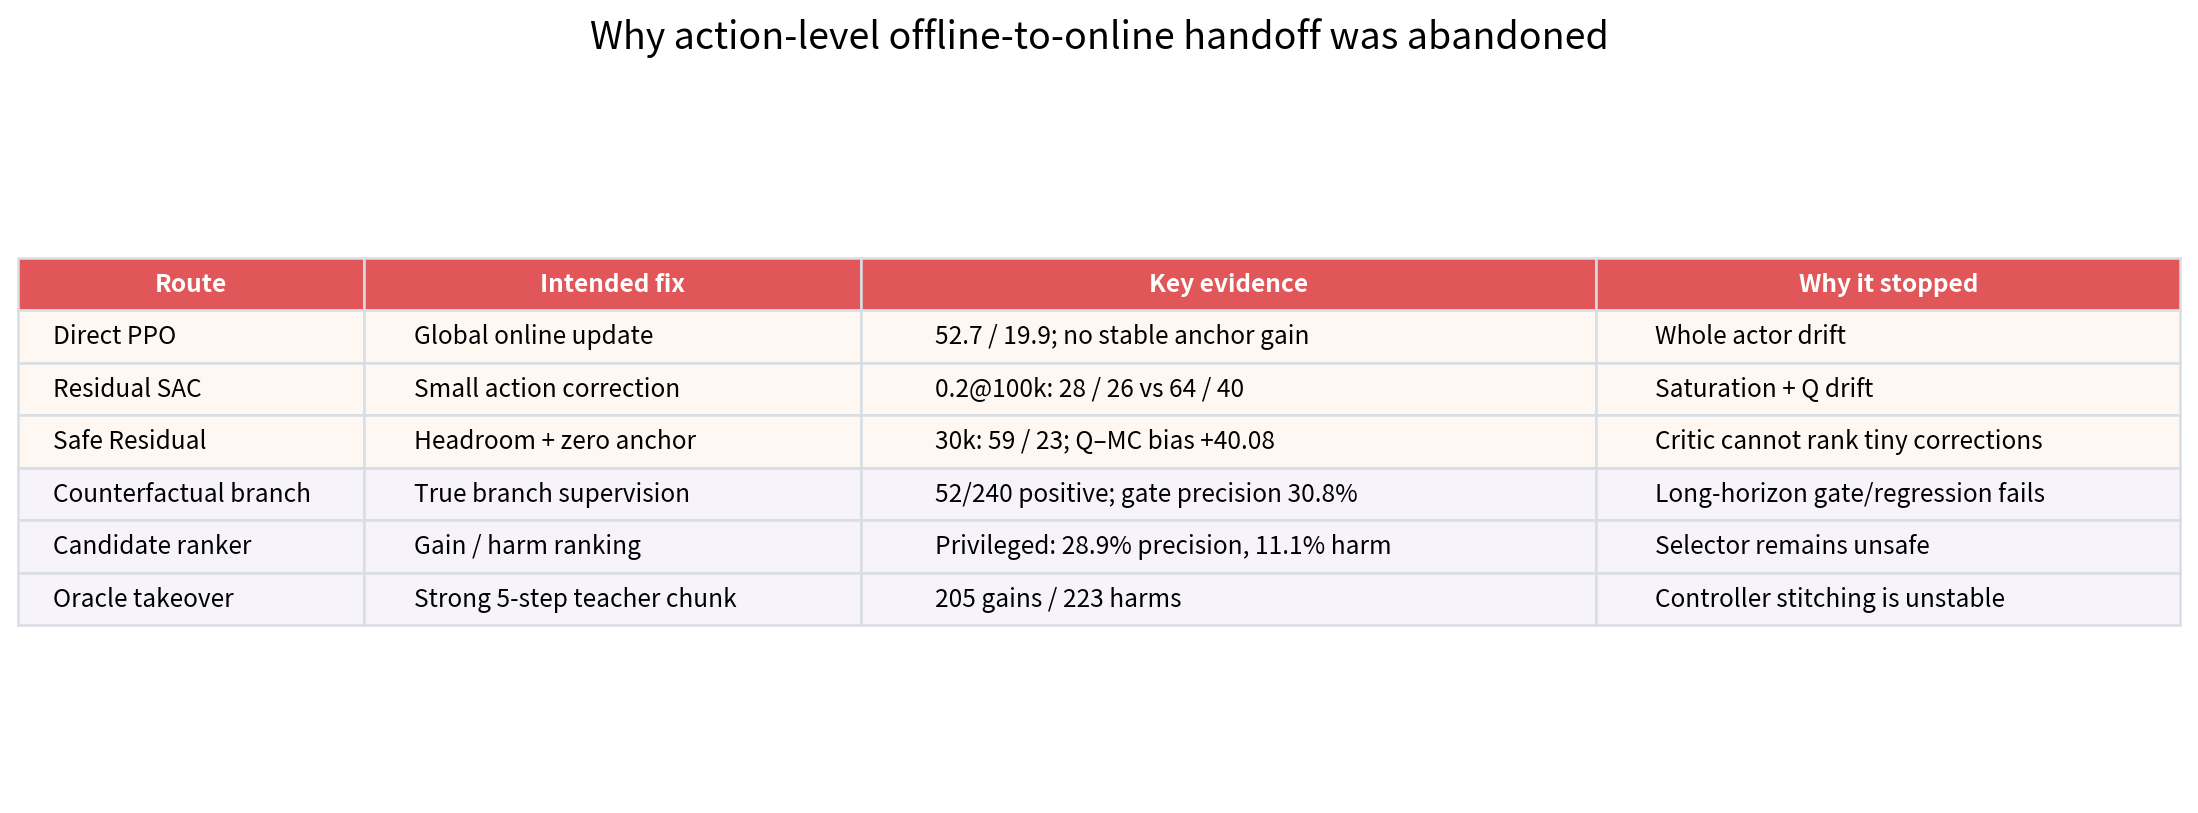
\includegraphics[width=\linewidth]{figures/05_failure_mechanisms.png}
\caption{Offline-to-online 失败机制总览}
\end{figure}

\textbf{图 5｜Offline-to-online 失败机制证据链。} 表中各行使用其各自固定开发协议，不能把百分比画成统一趋势；V2/V3 的 E0 bank、V4/V5 的 root branch 数据也不相同。数字用于定位停止原因，而非比较哪个版本``排名更高''。

\begin{longtable}[]{@{}
  >{\raggedright\arraybackslash}p{(\columnwidth - 6\tabcolsep) * \real{0.2500}}
  >{\raggedright\arraybackslash}p{(\columnwidth - 6\tabcolsep) * \real{0.2500}}
  >{\raggedright\arraybackslash}p{(\columnwidth - 6\tabcolsep) * \real{0.2500}}
  >{\raggedright\arraybackslash}p{(\columnwidth - 6\tabcolsep) * \real{0.2500}}@{}}
\toprule\noalign{}
\begin{minipage}[b]{\linewidth}\raggedright
路线
\end{minipage} & \begin{minipage}[b]{\linewidth}\raggedright
想解决的问题
\end{minipage} & \begin{minipage}[b]{\linewidth}\raggedright
关键实验结果
\end{minipage} & \begin{minipage}[b]{\linewidth}\raggedright
停止原因
\end{minipage} \\
\midrule\noalign{}
\endhead
\bottomrule\noalign{}
\endlastfoot
Direct PPO & 用 on-policy 数据提升整体策略 & checkpoint 经常在在线更新后退化，anchor 无稳定优势 & 完整 actor 漂移 \\
Residual SAC & 只在 AWAC 动作附近修正 & scale 0.2 在同一 50-episode bank 从 64/40 降到 28/26 & hard clip、residual saturation、Q drift \\
Safe Residual & 用 headroom、低熵和 zero anchor 保守交接 & 30k 为 59/23 对 62/34；correction 很小但 Q--MC bias 到 +40.08 & critic 无法可靠排序微小 correction \\
Counterfactual branch & 用真实同状态分支结果替代 Q 标签 & 52/240 roots 可改善，pending-exit 为 48.3\% & frozen-visual gate 与单一 winner 回归失败 \\
Candidate ranker & 使用全部候选的 gain/harm 标签 & privileged selector 仍只有 28.9\% precision、11.1\% harm & 长时 gain/harm 难以安全预测 \\
Oracle takeover & 用强 teacher 提供短动作 chunk & 1,200 roots 中 205 gain、223 harm & controller stitching 不稳定 \\
\end{longtable}

\hypertarget{ux5c0fux52a8ux4f5cux4e3aux4ec0ux4e48ux4f1aux88abux95edux73afux653eux5927}{%
\subsection{小动作为什么会被闭环放大}\label{ux5c0fux52a8ux4f5cux4e3aux4ec0ux4e48ux4f1aux88abux95edux73afux653eux5927}}

普通连续控制任务中，残差幅度小通常意味着安全；Adroit 接触任务不满足这一近似。设基础动作和残差组合为 \(a_t=a_t^{\text{base}}+\delta_t\)。即使 \(\lVert\delta_t\rVert\) 很小，它也可能改变接触法向力、滑移方向或某个手指是否保持接触。下一时刻 observation 由非线性动力学 \(s_{t+1}=f(s_t,a_t,c_t)\) 决定，其中接触模式 \(c_t\) 可以离散切换；一旦进入不同接触分支，后续 Frozen AWAC 面对的状态分布也随之改变。因此，``动作空间离基础策略近''不等价于``轨迹空间离基础策略近''。

V2 的 Residual SAC 使用完整执行动作训练 twin Q，并混合 50\% offline 与 50\% online replay，但 hard clip 让 residual 的概率语义和实际执行动作不一致；scale 0.2 的 action saturation 长期约 28\%，Q mean 最终升到约 610，同 bank 结果从 Frozen AWAC 的 64\% / 40\% 降到 28\% / 26\%。缩小到 0.1 只延缓退化：40k 一度为 64\% / 34\%，100k 仍降到 52\% / 20\%。因此不能选择性汇报 40k 的偶然最好点。

V3 用 action headroom 参数化消除了这一工程问题：残差只占基础动作到相应边界的比例，数值 clamp 为 0，\texttt{\textbar{}z\textbar{}\textgreater{}0.95} 比例为 0，per-dimension correction RMS 仅 0.0051，新增 boundary rate 约 0.071\%。然而 Safe Residual 在 30k 仍从 E0 的 62\% / 34\% 退到 59\% / 23\%。更关键的是，Q base 约 62.16，而同一 rollout 的 scaled Monte Carlo return 约 22.08，bias 从 10k 的约 +5.04 扩大到 +40.08，MAE 约 47.07。这排除了``大 residual 和硬裁剪是唯一原因''：即使动作足够小，错误的 Q 排序也会稳定推动 actor 朝坏方向更新。

\autocite{haarnoja2018sac}
